%%%%%%%%%%%%%%%%%%%%%%%%%%%%%%%%%%%%%%%%%%%%%%%%%%%%%%%%%%%%%%%%%%%%%%
%   長野高専電子情報工学科 卒業論文テンプレート
%
%   Original by Takuma Yoshida, 2010
%   Modified by Shoichi Ito, 2014-
%
%%%%%%%%%%%%%%%%%%%%%%%%%%%%%%%%%%%%%%%%%%%%%%%%%%%%%%%%%%%%%%%%%%%%%%

% 卒業論文スタイルファイルの適用([a4,11pt]のようなオプションは不要)
\documentclass{eithesis}

% よくつかうパッケージの読み込み
\usepackage{verbatim}
\usepackage{fancybox}
\usepackage{subcaption}
\usepackage{graphicx}
\usepackage{courier}
\usepackage{url}
\usepackage{fancyhdr}

\begin{document}
%%%%%%%%%%%%%%%%%%%%%%%%%%%%%%%%%%%%%%%%%%%%%%%%%%%%%%%%%%%%%%%%%%%%%%
%   表紙の設定
%%%%%%%%%%%%%%%%%%%%%%%%%%%%%%%%%%%%%%%%%%%%%%%%%%%%%%%%%%%%%%%%%%%%%%
\etGengou{令和元年度}      % 年度
\etTitle{Deep Learningを用いた天気予測}     % 論文タイトル(日本語)
\etTitleEn{Weather forecast using Deep Learning}    % 論文タイトル(英語)
\etDate{令和2年2月17日}   % 提出日(1月以降は年に注意)
\etAuthor{清水 翔仁}       % 著者フルネーム
\etLabName{西村研究室}     % 研究室名
\etMyProfessor{西村 治}    % 指導教員フルネーム
\etMakeTitle
%%%%%%%%%%%%%%%%%%%%%%%%%%%%%%%%%%%%%%%%%%%%%%%%%%%%%%%%%%%%%%%%%%%%%%
%   目次の出力
%%%%%%%%%%%%%%%%%%%%%%%%%%%%%%%%%%%%%%%%%%%%%%%%%%%%%%%%%%%%%%%%%%%%%%
\pagenumbering{roman}
\tableofcontents
\clearpage
\pagenumbering{arabic}
%%%%%%%%%%%%%%%%%%%%%%%%%%%%%%%%%%%%%%%%%%%%%%%%%%%%%%%%%%%%%%%%%%%%%%
%   ヘッダー・フッターの設定
%%%%%%%%%%%%%%%%%%%%%%%%%%%%%%%%%%%%%%%%%%%%%%%%%%%%%%%%%%%%%%%%%%%%%%
\pagestyle{fancyplain}
\lhead{\leftmark}  % ヘッダー左側(\leftmarkのデフォルトはsectionhead)
\chead{}           % ヘッダー中央
\rhead{\rightmark} % ヘッダー右側(\rightmarkのデフォルトはchapterhead)
\lfoot{}           % フッター左側
\cfoot{\thepage}   % フッター中央(ページ番号)
\rfoot{}           % フッター右側

%%%%%%%%%%%%%%%%%%%%%%%%%%%%%%%%%%%%%%%%%%%%%%%%%%%%%%%%%%%%%%%%%%%%%%
%   論文本体
%%%%%%%%%%%%%%%%%%%%%%%%%%%%%%%%%%%%%%%%%%%%%%%%%%%%%%%%%%%%%%%%%%%%%%
\chapter{はじめに}
	% ここで,論文で採りあげていることについて,
	% 現状・問題意識・それが解決するとどんないいことがあるか
	% などについてデータを並べながら説明する.
	% 最後に,論文全体の構成(2章では○○について述べ,3章では・・・)を書く.
	% 全体で1〜2ページ.
	現在の情報技術は,第四次産業革命とも呼ばれるほど大きな変化をもたらすと捉えられている.特に「人工知能(AI)」は,火薬と核兵器に次ぐ人類最大の発明とも称され,私達の将来を左右する力を持つと考えられる.また2000年代に「Deep Learning」の手法が開発されて以来,第三次AIブームが起こり,現在も進行中である.

	AI自らが知識を獲得することを「機械学習」という.Deep Learningは,機械学習の一種であるが,ニューラルネットワーク(NN)と呼ばれる人間の脳のメカニズム同様,大量の情報を多層的に処理する手法を用いる点が,従来の機械学習と異なっている.その多層的な情報処理の能力は,注目すべき点である特徴量を人間に支持されなくとも自ら見つけ出すことができる.したがってDeep Learningは,人間が従来認識していなかったような注目点や重要度を提示して「これが知である」という定義を行うことにより,人間の知能を超える可能性を持っている.\cite{rinri}

	Deep Learning技術は画像認識の分野をはじめとして,音声認識,自然言語処理の分野で大きな成果をあげているが,近年では気象予測の分野でもその適用例が報告されている.文献\cite{kishow}によると,現在気象庁が行っている天気予報では,「数値予報ガイダンス」と呼ばれる手法が使われている.数値予報ガイダンスとは,\figref{fig_guidance}のように,まず気象観測データから物理学の方程式を用いて風や気温などの時間変化を計算する.この計算によって得られた予測結果を数値予報モデルという.その後,予測結果を機械学習を用いて翻訳・修正し,天気予報の精度向上を図る方法である.

	この方法では,機械学習の入力となるのは,数値予報モデルから得られた未来の観測データである.また,天気の予測自体には機械学習を使用していない.そこで本研究では,過去の気象観測データを入力データとし,機械学習を用いて翌日の降水量の有無を予測する.
	\begin{figure}[htbp]
		\centering
		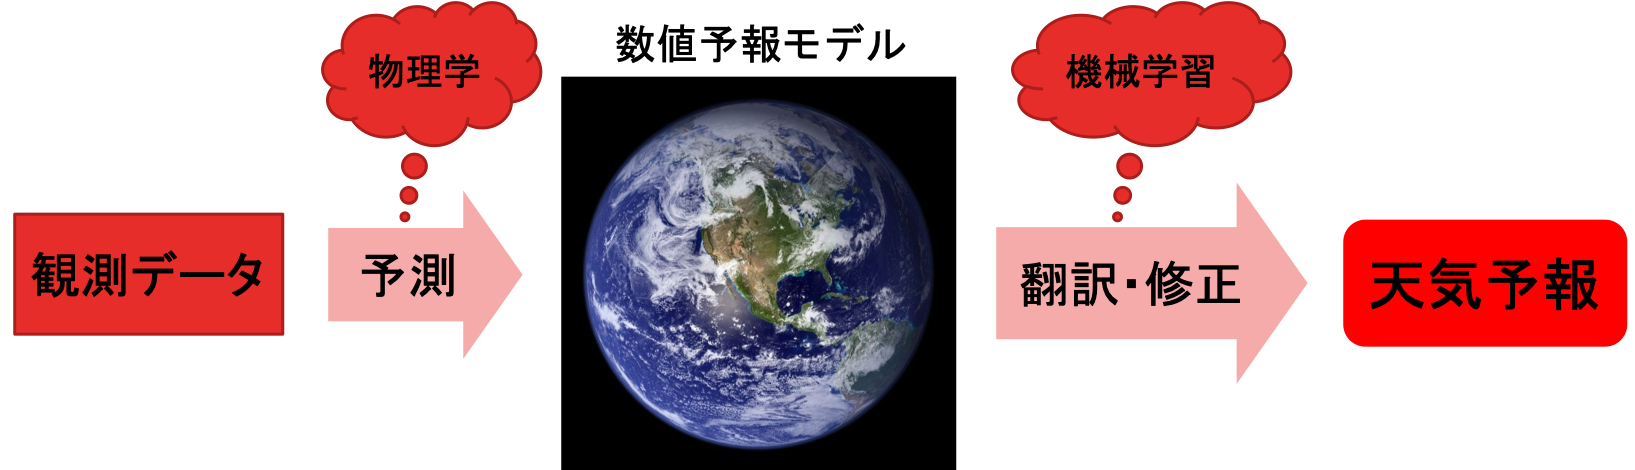
\includegraphics[width=14cm]{./images/guidance.png}
		\caption{数値予報ガイダンスの模式図}
		\label{fig_guidance}
	\end{figure}
	\clearpage

\chapter{原理}
	本章では,本研究で用いた手法の原理について説明する.

	\section{RNN(Recurrent Neural Network)}
		RNNとは,Deep Learningの手法の一種であり,時系列データの分析に特化している.\figref{fig_RNN}に,RNNの模式図を示す.ここで,$x_t$を時刻$t$におけるRNNの入力,$h_t$を時刻$t$におけるRNNの出力とする.
		\begin{figure}[htbp]
			\centering
			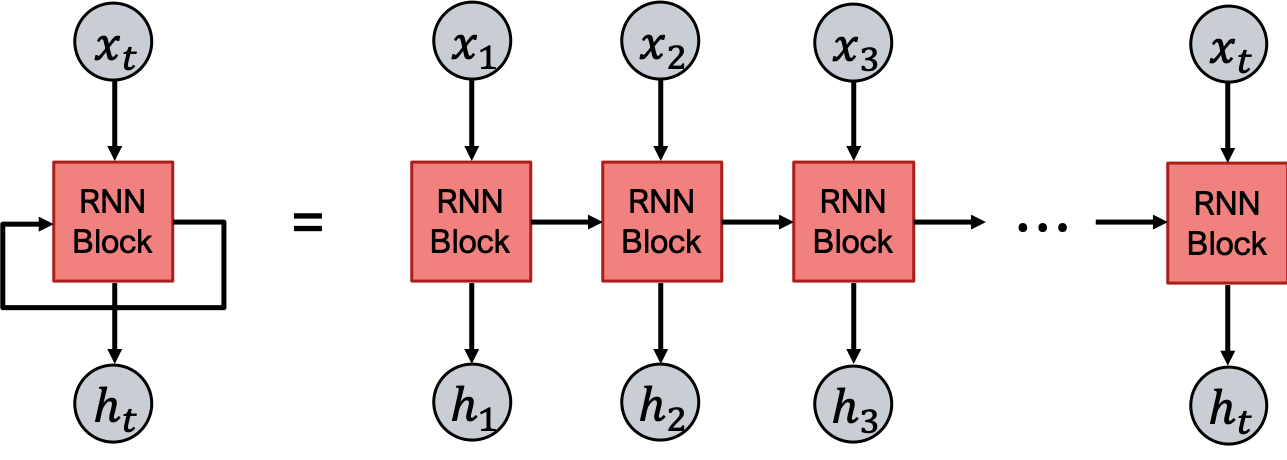
\includegraphics[width=14cm]{./images/RNN.png}
			\caption{展開されたRNN}
			\label{fig_RNN}
		\end{figure}

		\figref{fig_RNN}のように,RNNは内部にループ構造を持っている.これにより,前のステップでの分析結果を記憶し,データの時系列を理解することができる.しかし,RNNには長期依存性問題という欠点がある.長期依存性問題とは,記憶するステップ数が膨大になると計算が爆発するという問題である.そのため,現在単純なRNNはあまり使用されていない.

	\section{LSTM(Long Short Term Memory)}
		LSTMとは,RNNの長期依存性問題を解決した手法である.\figref{fig_RNN_inner}にRNNの内部を,\figref{fig_LSTM_inner}にLSTMの内部を示す.このとき,$\sigma$は0〜1を出力する関数,tanhは-1〜1を出力する関数とする.
		\begin{figure}[htbp]
			\centering
			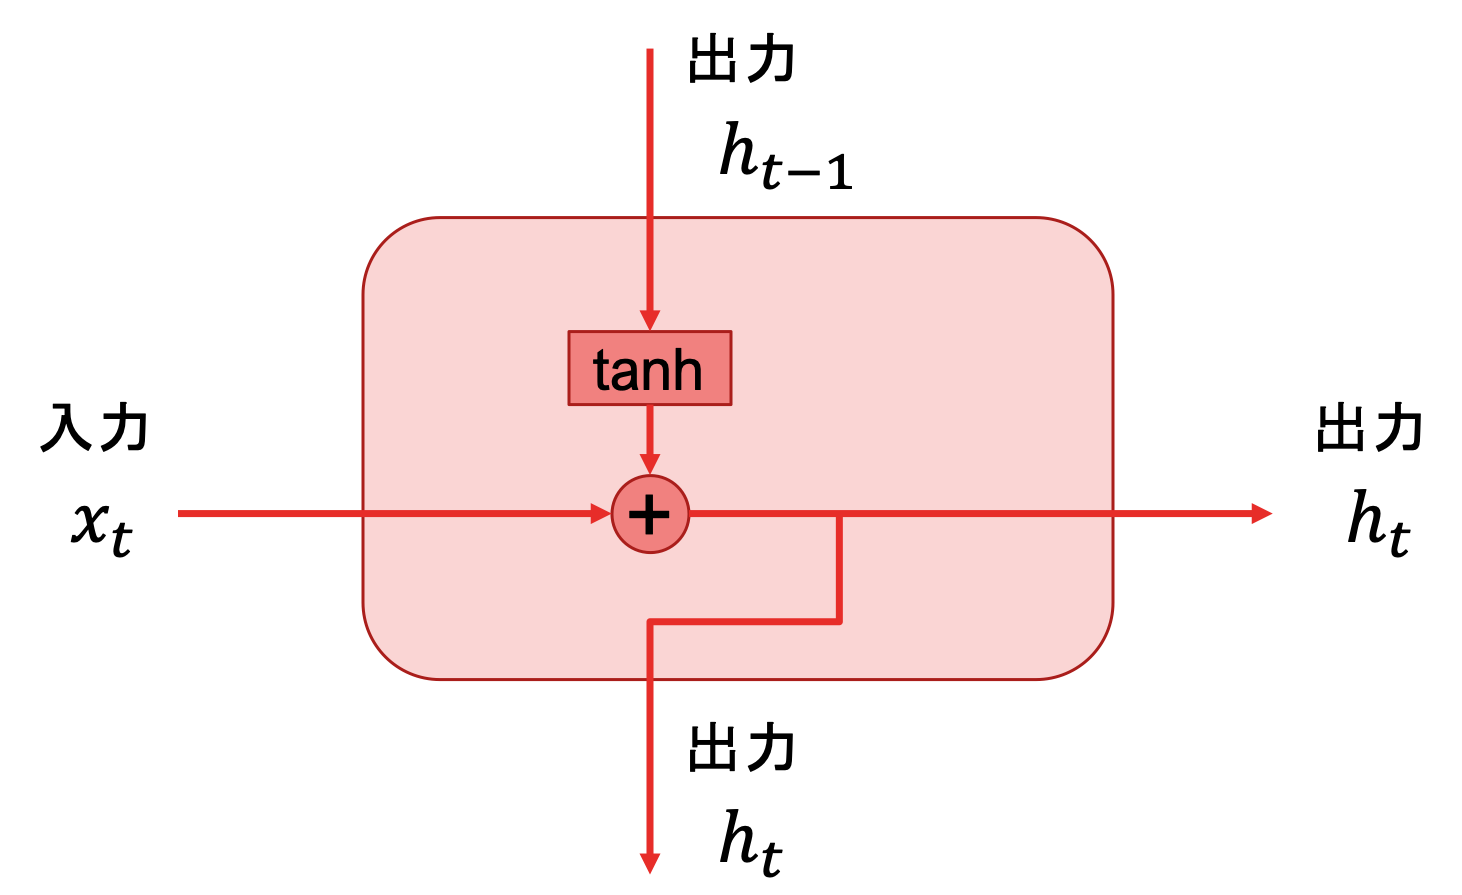
\includegraphics[width=14cm]{./images/RNN_inner.png}
			\caption{RNNの内部}
			\label{fig_RNN_inner}
		\end{figure}
		\begin{figure}[htbp]
			\centering
			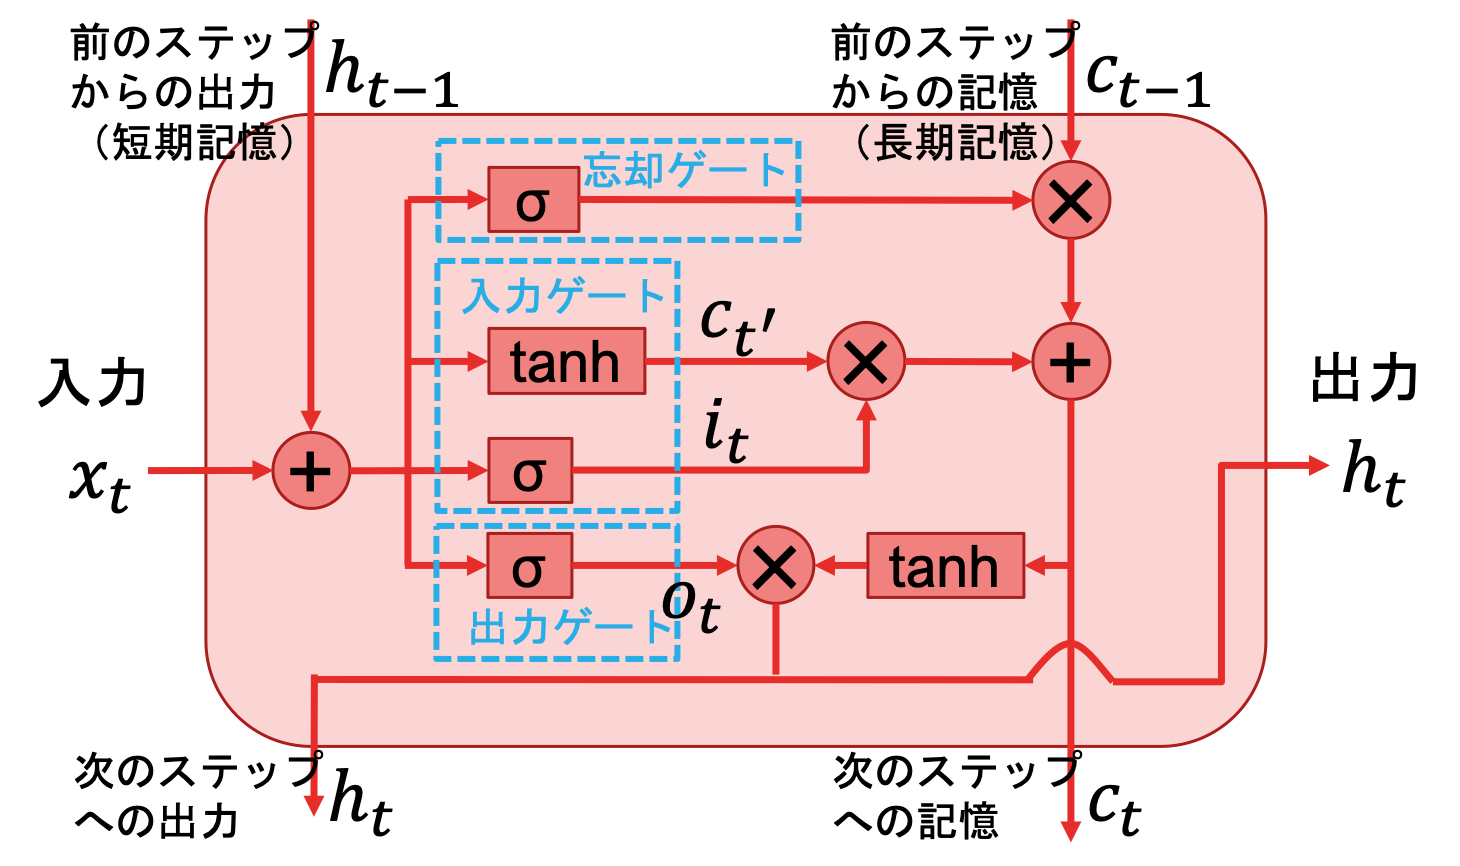
\includegraphics[width=14cm]{./images/LSTM_inner.png}
			\caption{LSTMの内部}
			\label{fig_LSTM_inner}
		\end{figure}

		\figref{fig_RNN_inner},\figref{fig_LSTM_inner}より,RNNは単一のtanh関数という非常に単純な構造に比べ,LSTMは4つの関数を含む複雑な構造をしている.
		
		ここで,\figref{fig_LSTM_inner}のLSTM内にデータが流れる手順について説明する.
		\begin{enumerate}
			\item 前のステップからの出力$h_{t-1}$と入力$x_t$が合流する.合流した信号はコピーされて4つのラインに分岐する.
			\item 一番上のラインの忘却ゲートでは,前のステップからの記憶一つ一つに対して,$\sigma$関数からの0〜1の値によって情報の取捨選択を行う.このとき1は情報を全て残し,0は全て捨てる.これにより,不要と思われる情報を捨てることで計算の爆発を防ぐ.
			\item 入力ゲートにおいて,前のステップからの出力$h_{t-1}$と入力$x_t$の合算を長期保存用に変換した上で,どの信号をどのくらいの重みで記憶に保存するか制御する.これは2つの手順で処理する.
				\begin{enumerate}
					\item tanh関数を用いて,入ってきた情報の情報量を削減し,必要な情報だけに変換された$c_{t'}$が出力する.
					\item $\sigma$関数の出力$i_t$によって,$h_{t-1}$を考慮して入力$x_t$の重みを調整する.
				\end{enumerate}
			\item 出力ゲートにおいて,上記の処理で取捨選択された長期記憶$c_t$の中で,短期記憶$h_t$に関する部分のみを出力する.これも2つの手順で処理する.
				\begin{enumerate}
					\item 前のステップからの記憶$c_{t-1}$と,入力$x_t$を変換した短期記憶$c_{t'}$を合算し,長期記憶$c_t$として出力する.これは,それぞれ既に忘却ゲートおよび入力ゲートで取捨選択が行われている.
					\item tanh関数に$c_t$を入力したものに対し,$\sigma$関数からの0〜1の値$o_t$によって情報の取捨選択を行う.
				\end{enumerate}
		\end{enumerate}

\chapter{予備知識}
	% 章の最初には,その章を簡潔にまとめた数行のリード文を入れ,
	% その章を読むべきかどうかの判断材料を読者に与える.
	本章では,本研究を説明する上で必要な用語について述べる.

	\section{モデル}
		モデルとは,コンピュータが分かる形の入力値を受け取り,何かしらの評価・判定をして出力値を出すものである.機械学習やAIにおいて中心的な役割を担う頭脳を意味する.
	\section{エポック数}
		エポック数とは,モデルが学習データセットに対して学習した回数である.エポック数が多すぎると「過学習」を起こし,正確な結果が得られない.逆に少なすぎると,モデルの学習が足りないため精度が伸びない.
	\section{過学習}
		過学習とは,トレーニングデータセットではうまく機能するモデルが,未知のデータ(テストデータセット)ではうまく汎化されないという問題のことである.その原因は,データに対してモデルが複雑過ぎることや,トレーニングデータセットが足りないことによる学習不足だと考えられる.経験則として,学習中にテストデータの損失が一旦下がったあとに増加したら,それは過学習を起こしている兆候である.\cite{oreilly}
	\section{隠れ層}
		隠れ層とは,ニューラルネットワークにおける入力層と出力層以外の層のことである.一般に,隠れ層の数や,一つの層あたりのノード数が多ければ多いほど精度が高くなる.しかし多すぎるとモデルが複雑になってしまい,過学習を引き起こす.
	\section{バッチサイズ}
		学習データセットをいくつかに小分けしたかたまりのことをバッチといい,その大きさのことをバッチサイズという.
	\section{正規化}
		機械学習では,学習データのそれぞれの値によって大きく桁が異なると,良い性能が得られないという性質がある.そこでデータの値をすべて0〜1の間に収めることを正規化という.サンプル$x^{\left( i\right) }$の正規化した値$x^{\left( i\right) }_{norm}$を求める式を式(\ref{eq_norm})に示す.式(\ref{eq_norm})において,$x^{\left( i\right) }$は特定のサンプルであり,$x^{\left( i\right) }_{min}$は特徴量の列における最小値,$x^{\left( i\right) }_{\max}$は最大値を表す.\cite{python}
		\begin{equation}\label{eq_norm}
			x^{\left( i\right) }_{norm}=\dfrac {x^{\left( i\right) }-x_{\min }}{x_{\max }-x_{\min }}
		\end{equation}

\chapter{実装方法}
	本章では,開発環境や精度向上のために行ったことについて説明する.

	\section{開発環境}
		本研究の開発環境を\tabref{tab_environment}に示す.
		\begin{table}[htbp]
			\centering 
			\caption{開発環境}
			\label{tab_environment}
			\begin{tabular}{c|c}
				\toprule
				OS & macOS Catalina 10.15.2 \\
				CPU & Intel(R) Core i7-5650U CPU@2.20GHz \\
				プログラミング言語 & Python 3.7.4 \\
				ニューラルネットワークライブラリ & keras 2.3.1 \\
				デバッグツール & TensorBoard 2.1.0 \\
				\bottomrule
			\end{tabular}
		\end{table}

	\section{学習データセット}
		今回の学習データセットは,気象庁ホームページ\cite{data}にて公開されている気象観測データをダウンロードして使用する.ダウンロードするにあたって指定した条件を以下に示す.
		\begin{itemize}
			\item データ形式:CSV
			\item 期間:1998/1/1 - 2019/12/31
			\item 地点:長野市
			\item 特徴量:日平均現地気圧,日平均気温,日最低気温,日最高気温,降水量の日合計,日照時間,日平均風速,日最大風速,日平均相対湿度,日最小相対湿度,日平均雲量
		\end{itemize}

		次に,実際にダウンロードしたデータの例を\tabref{tab_sample}に示す.\tabref{tab_sample}より,この状態では気圧の値のみが明らかに桁が大きいため,全体に正規化の処理を施す.
		\begin{table}[htbp]
			\centering 
			\caption{学習データの例}
			\label{tab_sample}
			\begin{tabular}[htbp]{c|c|c|c|c}
				日付 & 気圧[hPa] & 平均気温[$^\circ$C] & 最高気温[$^\circ$C] & 最低気温[$^\circ$C] \\ \hline
				1998/1/1 & 965.8 & 0.4 & 5.5 & -3.9 \\
				1998/1/2 & 968.3 & 3.2 & 8.0 &  0.0 \\
				1998/1/3 & 969.9 & 2.3 & 9.8 & -3.0 \\
				1998/1/4 & 960.8 & 3.2 & 9.7 & -1.1 \\
			\end{tabular}
		\end{table}

		\tabref{tab_sample}の値を正規化したものを\tabref{tab_sample_norm}に示す.\tabref{tab_sample_norm}より,全ての値が0〜1の間に収まっており,大小関係も変化していないことがわかる.
		\begin{table}[htbp]
			\centering 
			\caption{正規化後の学習データ}
			\label{tab_sample_norm}
			\begin{tabular}[htbp]{c|c|c|c|c}
				日付 & 気圧 & 平均気温 & 最高気温 & 最低気温 \\ \hline
				1998/1/1 & 0.618 & 0.189 & 0.218 & 0.205 \\
				1998/1/2 & 0.670 & 0.263 & 0.277 & 0.303 \\
				1998/1/3 & 0.704 & 0.239 & 0.320 & 0.227 \\
				1998/1/4 & 0.514 & 0.263 & 0.318 & 0.275 \\
			\end{tabular}
		\end{table}

\chapter{結果}
	ここでは,隠れ層の数によって予測の精度がどの程度向上するのかを調べるため,隠れ層の数が1つの場合,2つの場合,3つの場合の3パターンについてプログラムを実行する.

	まず隠れ層が1つの場合についての結果を\figref{fig_hidden1_acc},\figref{fig_hidden1_loss}に示す.\figref{fig_hidden1_acc}より,精度が右肩上がりに上昇し,90\%近くに達していることがわかる.また\figref{fig_hidden1_loss}より,損失が右肩下がりに減少し,値が0.25ほどになっていることがわかる.
	\begin{figure}[htbp]
		\centering
		\fbox{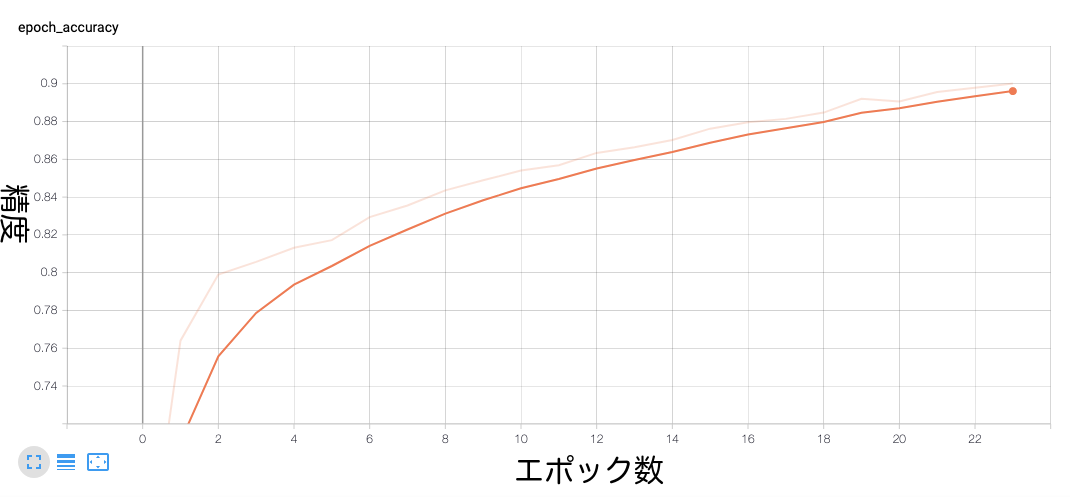
\includegraphics[width=14cm]{./images/hidden1_acc_v3.png}}
		\caption{隠れ層が1つの場合の精度}
		\label{fig_hidden1_acc}
	\end{figure}
	\begin{figure}[htbp]
		\centering
		\fbox{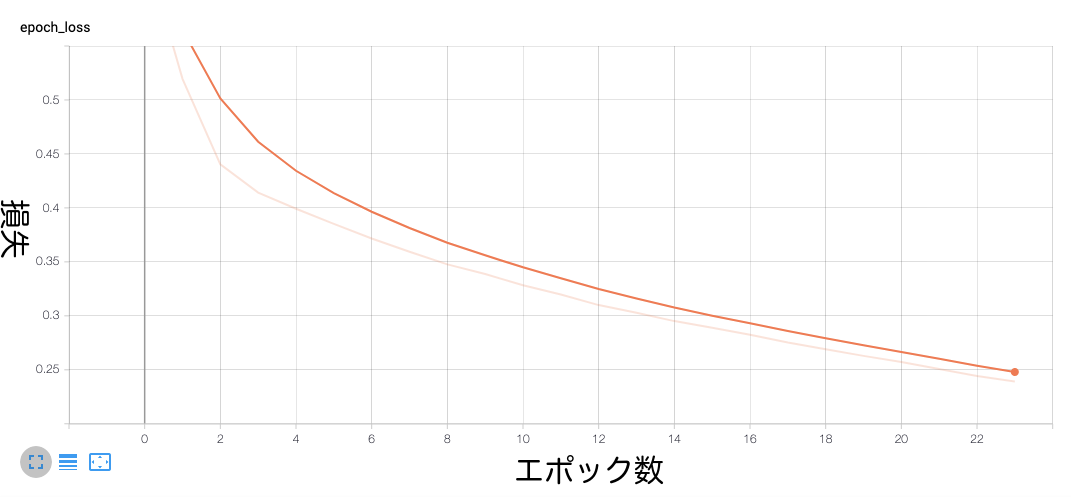
\includegraphics[width=14cm]{./images/hidden1_loss_v3.png}}
		\caption{隠れ層が1つの場合の損失}
		\label{fig_hidden1_loss}
	\end{figure}

	次に隠れ層が2つの場合についての結果を\figref{fig_hidden2_acc},\figref{fig_hidden2_loss}に示す.\figref{fig_hidden2_acc}より,精度が99\%に達し\figref{fig_hidden1_acc}よりも高い精度が得られている.また\figref{fig_hidden2_loss}より,損失が0に近い値になり\figref{fig_hidden1_loss}よりも減少していることがわかる.このことから,隠れ層の数を増やすことが精度向上に寄与していると考えられる.
	\begin{figure}[htbp]
		\centering
		\fbox{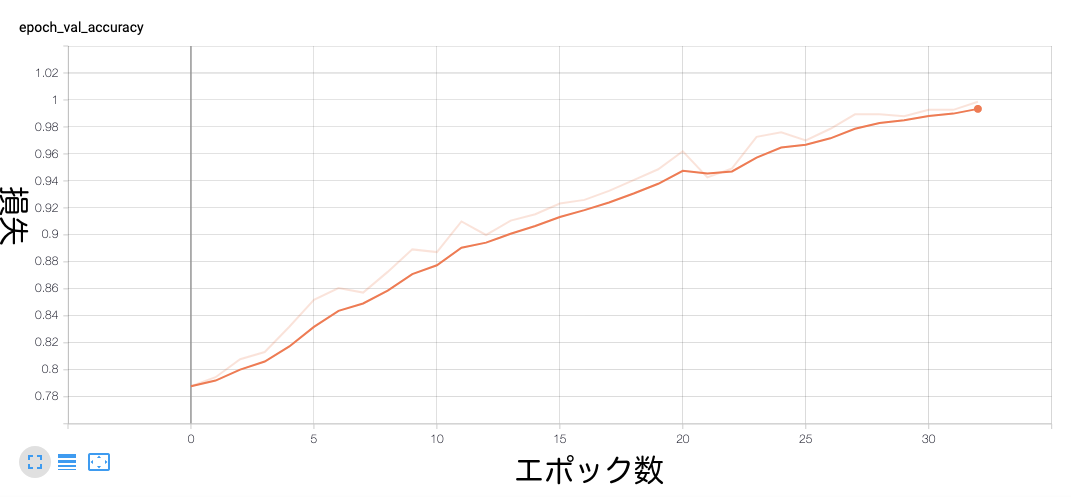
\includegraphics[width=14cm]{./images/hidden2_acc_v2.png}}
		\caption{隠れ層が2つの場合の精度}
		\label{fig_hidden2_acc}
	\end{figure}
	\begin{figure}[htbp]
		\centering
		\fbox{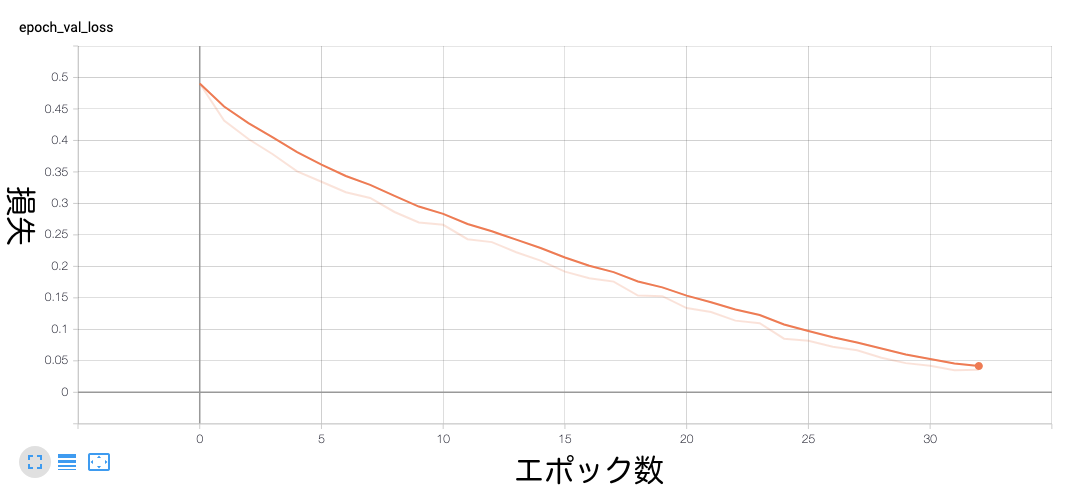
\includegraphics[width=14cm]{./images/hidden2_loss_v2.png}}
		\caption{隠れ層が2つの場合の損失}
		\label{fig_hidden2_loss}
	\end{figure}

	隠れ層が3つの場合についての結果を\figref{fig_hidden3_acc},\figref{fig_hidden3_loss}に示す.\figref{fig_hidden3_acc}より,エポック数が7の時点で精度の上昇が頭打ちになり,エポック数8で減少していることがわかる.また\figref{fig_hidden3_loss}より,下がっていた損失がエポック数7で上昇していることがわかる.このことから,隠れ層を増やしたことによりニューラルネットワークが複雑になり,過学習が発生していると考えられる.また,以上の結果から隠れ層の数は2つが適当であると考えられる.
	\begin{figure}[htbp]
		\centering
		\fbox{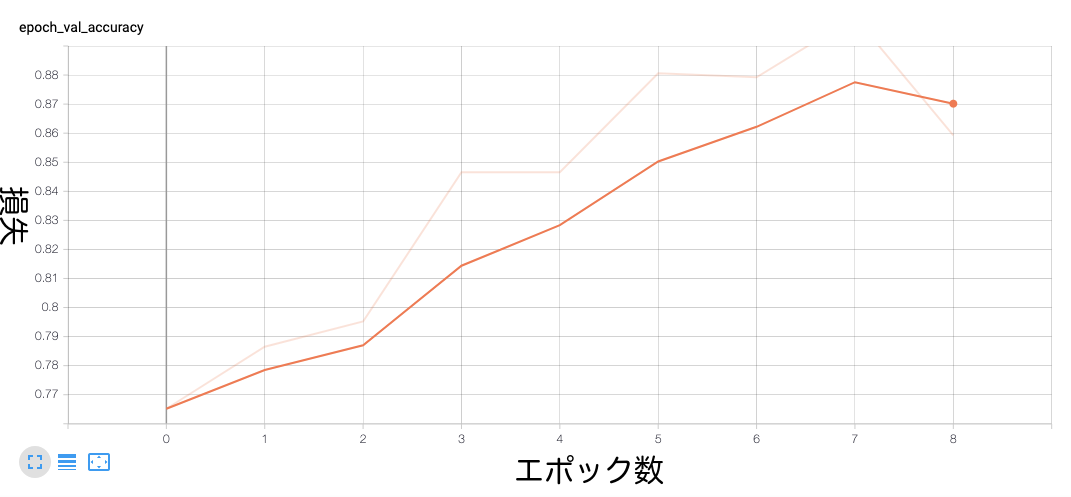
\includegraphics[width=14cm]{./images/hidden3_acc_v2.png}}
		\caption{隠れ層が3つの場合の精度}
		\label{fig_hidden3_acc}
	\end{figure}
	\begin{figure}[htbp]
		\centering
		\fbox{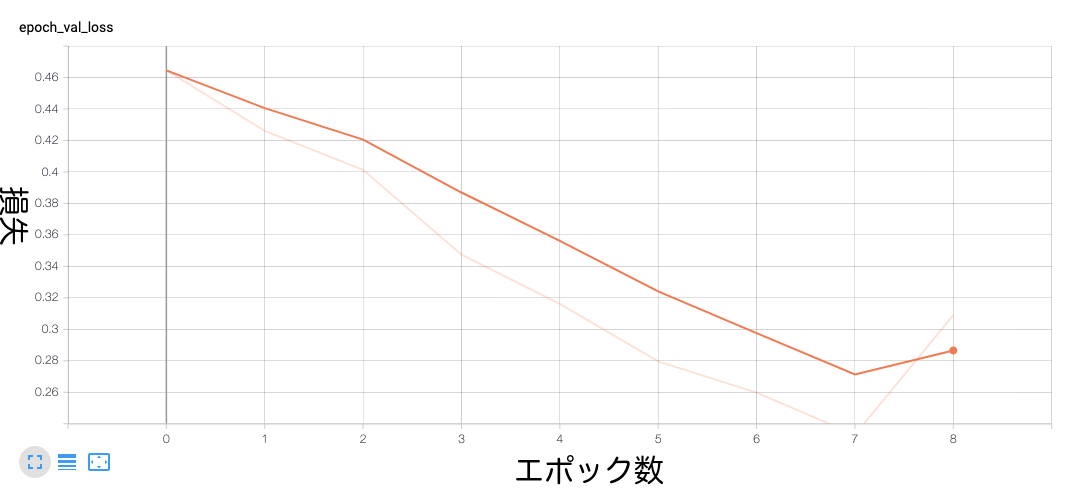
\includegraphics[width=14cm]{./images/hidden3_loss_v2.png}}
		\caption{隠れ層が3つの場合の損失}
		\label{fig_hidden3_loss}
	\end{figure}

	隠れ層の数を2つに固定し,プログラムを10回実行した際の精度を\tabref{tab_acc}に示す.\tabref{tab_acc}より,予測の精度は約94\%となった.よって,かなり高い精度で降水量の有無を予測できていると考えられる.
	\begin{table}[htbp]
		\centering 
		\caption{予測精度}
		\label{tab_acc}
		\begin{tabular}[htbp]{c|c}
			番号 & 精度 \\ \hline
			1 & 0.9248 \\
			2 & 0.9845 \\
			3 & 0.8873 \\
			4 & 0.9028 \\
			5 & 0.9521 \\
			6 & 0.9578 \\
			7 & 0.9560 \\
			8 & 0.9601 \\
			9 & 0.9380 \\
			10 & 0.9091 \\ \hline
			平均 & 0.93725
		\end{tabular}
	\end{table}

\chapter{まとめ}
	% 「はじめに」で振った話や問題意識がどれだけ回収できているか,
	% なにが問題として残ったのか.
	% あらためて研究のはじめから終わりまでの全体を俯瞰してのまとめを書く.
	% どうせやる予定のない「今後の予定」は書いてはいけない.
	本研究の目標である,過去の気象観測データから翌日の降水量の有無を予測することができた.
	また研究を進める中で,機械学習を行うプログラムの,実装方法を学ぶことができた.

	改善点としては,現在日別に出力している予測結果を,より詳細な1時間毎の結果に拡大すること.
	そして降水の有無ではなく,どれくらい雨が降るか,というような降水量の予測を行うことが挙げられる.

%%%%%%%%%%%%%%%%%%%%%%%%%%%%%%%%%%%%%%%%%%%%%%%%%%%%%%%%%%%%%%%%%%%%%%
%   謝辞と参考文献
%%%%%%%%%%%%%%%%%%%%%%%%%%%%%%%%%%%%%%%%%%%%%%%%%%%%%%%%%%%%%%%%%%%%%%
\chapter*{謝辞}
	% ここは自由に書いて良い.その人の協力なくしてこの研究は成し遂げられなかった
	% と思われる人への謝意をあらわす.名前は基本的にフルネームで入れる.
	本研究を進めるに当たり,西村治教授から多大な助言を賜りました.厚く感謝を申し上げます.また一年間同じ研究室で研究を行ってきた青沼葵さん,櫻井優太さん,関谷賢二さん,山本七海さんにも感謝の意を表します.
	\begin{flushright}
		2020年2月

		清水翔仁
	\end{flushright}

\begin{thebibliography}{99}
\bibitem{rinri}{鬼頭 葉子: 技術者の倫理, ナカニシヤ出版, 2018.}
\bibitem{kishow}{気象庁 | 数値予報課報告・別冊第64号(令和2年2月16日現在): \url{https://www.jma.go.jp/jma/kishou/books/nwpreport/64/chapter1.pdf}}
\bibitem{data}{気象庁 | 過去の気象データ・ダウンロード(令和2年2月16日現在): \url{https://www.data.jma.go.jp/gmd/risk/obsdl/index.php}}
\bibitem{oreilly}{Antonio Gulli・Sujit Pal(著),大串正矢・久保隆宏・中山光樹(訳): 直感Deep Learning, 株式会社オライリー・ジャパン, 2019.}
\bibitem{python}{Sebastian Raschka・Vahid Mirjalili(著),株式会社クイープ(訳): [第2版]Python機械学習プログラミング, 株式会社インプレス, 2018.}
\bibitem{tb}{TensorBoard(令和2年1月20日現在): \url{https://www.tensorflow.org/tensorboard}}
\end{thebibliography}

%%%%%%%%%%%%%%%%%%%%%%%%%%%%%%%%%%%%%%%%%%%%%%%%%%%%%%%%%%%%%%%%%%%%%%
%   付録
%%%%%%%%%%%%%%%%%%%%%%%%%%%%%%%%%%%%%%%%%%%%%%%%%%%%%%%%%%%%%%%%%%%%%%
\appendix
\chapter{ソースコード}
	% 本編に入れると冗長になる式変形や,話の細かいところは
	% ここに入れる.研究に利用したソフトウェアのインストール方法や
	% コンパイル方法なども詳細に書いておくと親切であろう.
	本研究で実装したプログラムのソースコードをソースコード\ref{code}に示す.
	\lstinputlisting[caption=翌日の降水量の有無を予測するプログラム, label=code]{../precaution_v2.py}

\end{document}
